\begin{displayquote}
	\textsf{High-Performance Computing (HPC) most generally refers to the practice of aggregating computing power in a way that delivers much higher performance than one could get out of a typical desktop computer or workstation to solve large-scale problems in science, engineering, or business. HPC is one of the most active research areas in Computer Science because it is strategically essential to solve the large challenge problems arising from scientific and industrial applications. The development of HPC relies on the efforts from multi-disciplines, including the computer architecture design, the parallel algorithms, and programming models, etc. This chapter gives the state-of-the-art in HPC: its history of evolution, modern computing architectures, and parallel programming models. Finally, we discuss the critical challenges to the whole HPC community with the coming of exascale supercomputers.}
\end{displayquote}

\vspace{0.6in}

\section{Evolution of HPC}

The terms \textit{high-performance computing} and \textit{supercomputing} are sometimes used interchangeably. A supercomputer is a computing platform with a high level of performance, which is constructed by large numbers of computing units connected by a local high-speed computer bus. HPC technology is implemented in a wide range of computationally intensive applications in multidisciplinary areas including biosciences, geographical data, electronic design, climate research, neuroscience, quantum mechanics, molecular modeling, nuclear fusion, etc. Supercomputers were introduced in the 1960s, and the performance of a supercomputer is measured in floating-point operations per second (FLOPS). Since the first generation of supercomputers, the \textit{megascale} performance was reached in the 1970s, and the \textit{gigascale} performance was passed in less than ten years. Finally, the \textit{terascale} performance was achieved in the 1990s, and then the \textit{petascale} performance was crossed in 2008 with the installation IBM Roadrunner at Los Alamos National Laboratory in the United States. Fig. \ref{sc_evaluate} shows the Top 1 supercomputer's peak performance by year since the 1960s.

\begin{figure}[htbp]
	\centering
	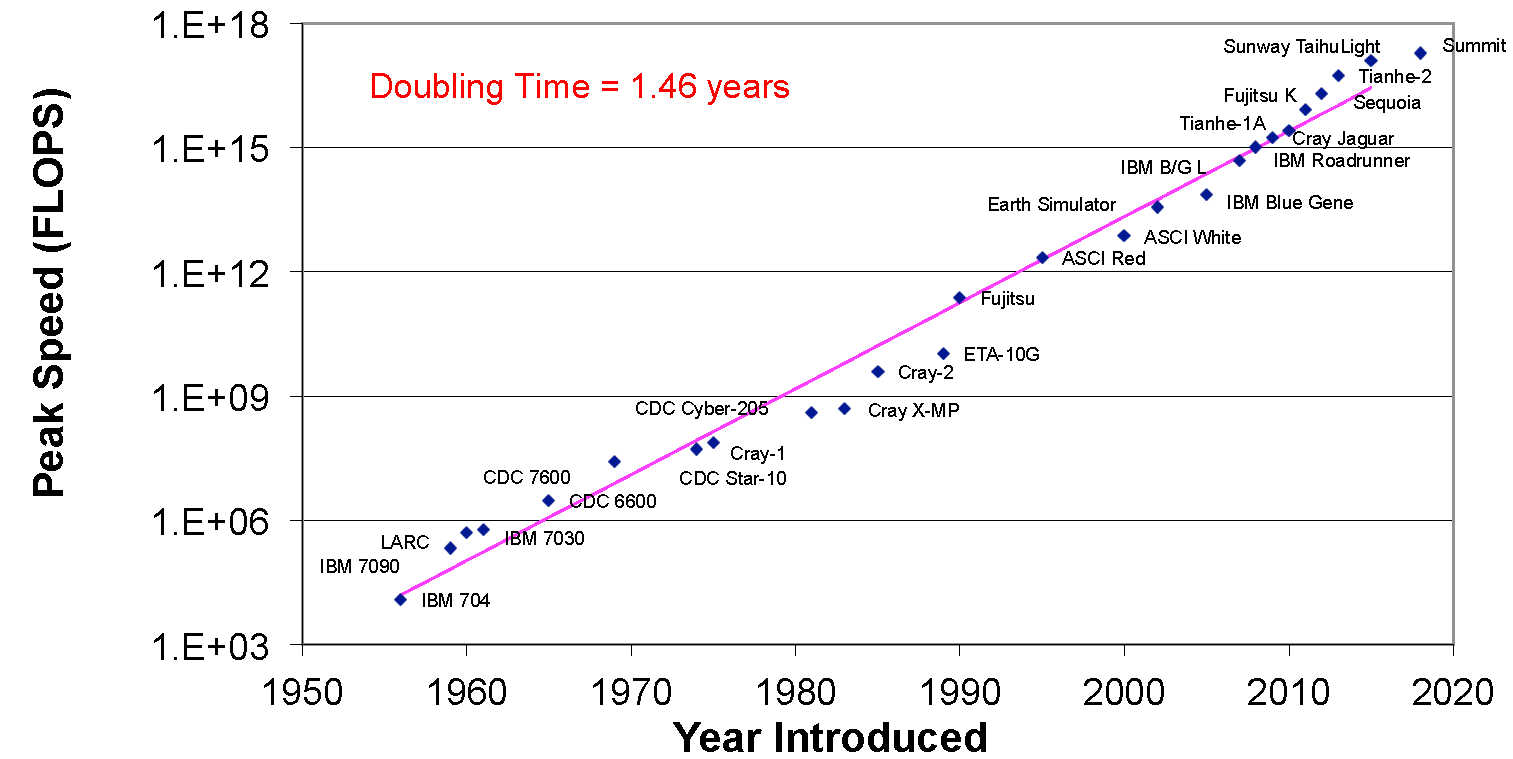
\includegraphics[width=0.99\linewidth]{fig/sc_evaluate.pdf}
	\caption{Top 1 Supercomputers' Performance by Year.}
	\label{sc_evaluate}
\end{figure}


Since 1993, the TOP500 project\footnote{https://www.top500.org} ranks and details the 500 most powerful supercomputing systems in the world and publishes an updated list of the supercomputers twice a year. The project aims to provide a reliable basis for tracking and detecting trends in HPC and bases rankings on HPL \cite{dongarra2003linpack}, a portable implementation of the high-performance LINPACK benchmark written in Fortran for distributed-memory computers. HPL is a software package that solves a (random) dense linear system in double precision (64 bits) arithmetic on distributed-memory computers. The algorithm used by HPL can be summarized by the following keywords: 
\begin{itemize}
	\item two-dimensional block-cyclic data distribution;
	\item right-looking variant of the LU factorization with row partial pivoting featuring multiple look-ahead depths;
	\item recursive panel factorization with pivot search and column broadcast combined;
	\item various virtual panel broadcast topologies;
	\item bandwidth reducing swap-broadcast algorithm;
	\item backward substitution with look-ahead of depth 1.
\end{itemize}

According to the newest Top500 list of November 2018, the fastest supercomputer is the Summit of the United States, which has a LINPACK benchmark score of 122.3 PFLOPS. The Sunway TaihuLight, Sierra and Tianhe-2A follow closely the Summit, with the performance respectively 93 PFLOPS, 71.6 PFLOPS, and 61.4 PFLOPS. Fig. \ref{hpl_by_year} gives the No. 1 machine of HPL performance by year since 1993.

\begin{figure}[t]
	\centering
	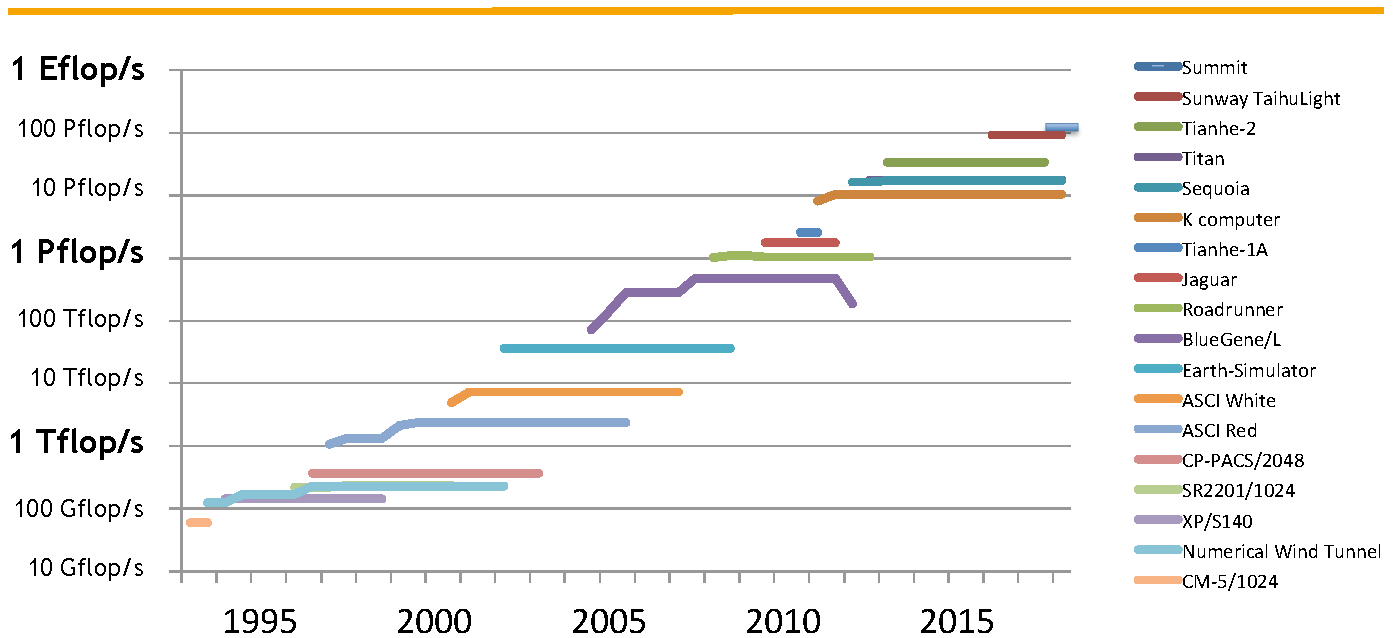
\includegraphics[width=6.3in]{fig/top500_3.pdf}
	\caption{No. 1 machine of HPL Performance by year.}
	\label{hpl_by_year}
\end{figure}

The next barrier for the HPC community to overcome is the \textit{exascale} computing, which refers to the computing systems capable of at least one exaFLOPS ($10^{18}$ floating point operations per second). This capacity represents a thousandfold increase over the first petascale computer which came into operation in 2008. The world first exascale supercomputer will come around 2020. China's first exascale supercomputer will enter service by 2020. United States's first exascale computer is planned to be built by 2021 at Argonne National Laboratory. The post-K announced by Japan will start the public service around 2021, and the first exascale supercomputer in Europe will appear around 2022. Exascale computing would be considered as a significant achievement in computer engineering, for it is estimated to be the order of processing power of the human brain at the neural level.

Considering the evolution of HPC, there are always two questions proposed to the users who want to develop the applications on supercomputers:

\begin{itemize}
	\item \textit{How to build such powerful supercomputers?}
	\item \textit{How to develop the applications to profit efficiently the total computational capacity of supercomputers?}
\end{itemize}

In order to answer these two questions above, firstly, Section \ref{Modern Computing Architectures} gives a glance at the modern computing architectures to build the supercomputers. Then different parallel programming models to develop the applications on the supercomputers are given in Section \ref{Parallel Programming Model}.


\section{Modern Computing Architectures}\label{Modern Computing Architectures}

Different architectures of computing units are designed to build the supercomputers. In this section, the state-of-the-art of modern CPUs and accelerators are reviewed.

\subsection{CPU Architectures and Memory Access}

The development of modern CPUs is based on the \textit{Von Neumann architecture}. The proposition of this computer architecture is based on the description by the mathematician and physicist \textit{John von Neumann} and others in the \textit{First Draft of a Report on the EDVAC} \cite{von1945first}. All the modern computing units are all envolved from this concept, which consists of five parts:

\begin{itemize}
	\item A \textit{processing unit} that contains an arithmetic logic unit and processor registers;
	\item A \textit{control unit} that contains an instruction register and program counter;
	\item \textit{Memory} that stores data and instructions;
	\item External mass \textit{storage};
	\item \textit{Input/output} mechanisms.
\end{itemize}

As shown in Fig. \ref{von-neumann}, the \textit{Von Neumann architecture} uses the shared bus between the program memory and data memory, which leads to its bottleneck. Since the single bus can only access one of the two types of memory at a time, the data transfer rate between the CPU and memory is rather low. With the increase of CPU speed and memory size,  the bottleneck has become more of a problem.

\begin{figure}[t]
	\centering
	\subfloat[Von Neumann architecture.]{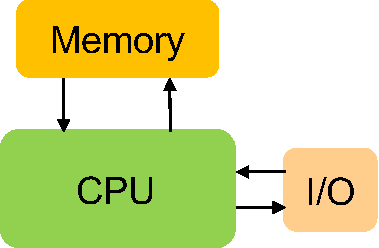
\includegraphics[width=0.31\linewidth]{fig/von-neumann.pdf}%
		\label{von-neumann}}
	\hspace{8.5pt}
	\subfloat[Harvard architecture.]{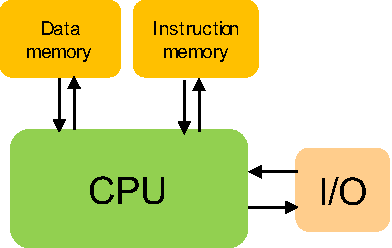
\includegraphics[width=0.31\linewidth]{fig/harvard.pdf}%
		\label{havard}}
	\hspace{8.5pt}
	\subfloat[Modified Harvard architecture.]{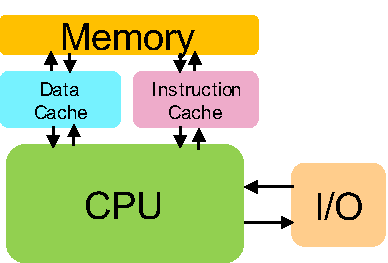
\includegraphics[width=0.31\linewidth]{fig/modified-harvard.pdf}%
	\label{modified-havard}}
	\caption{ Computer architectures.}
	\label{cpu-arch}
\end{figure}

The \textit{Harvard architecture} is another computer architecture with physically separate the storage and bus for the instructions and data. As shown in Fig. \ref{havard}, the limitation of a pure Harvard architecture is that the mechanisms must be provided to load the program to be executed into instruction memory separately and any data to be operated upon input memory. Additionally, read-only technology for the instruction memory allows the computer to begin execution of a pre-loaded program as soon as power is applied. The data memory will at this time be in an unknown state, so it is not possible to provide any kind of pre-defined data values to the program.

Today, most processors implement the separate pathways as \textit{Harvard architecture} to support the higher performance concurrent data and instruction access, meanwhile loosen the strictly separated storage between code and data. That is named as the \textit{Modified Havard architecture} (shown as Fig. \ref{modified-havard}). This model can be seen as the combination of the \textit{Von Neumann architecture} and  \textit{Harvard architecture}.

The solution is to provide a hardware pathway and machine language instructions so that the contents of the instruction memory can be read as if they were data. Initial data values can then be copied from the instruction memory into data memory when the program starts. If the data is not to be modified, it can be accessed by the running program directly from instruction memory without taking up space in the data memory.

Nowadays, most CPUs have Von Neumann like unified address space and also separate instruction and data caches as well as memory protection, making them more Harvard-like, and so they could be classified more as \textit{modified Harvard architecture} even using unified address space.

\begin{figure}[htbp]
	\centering
	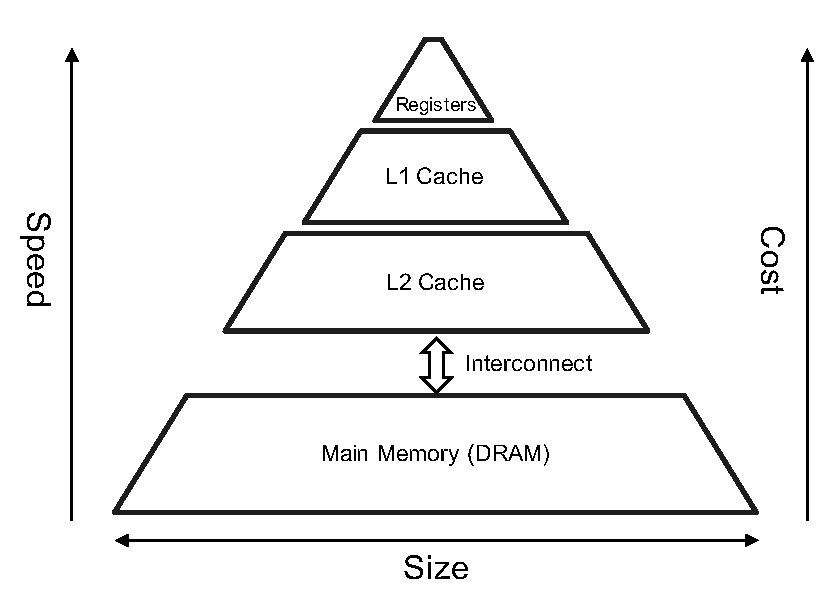
\includegraphics[width=0.81\linewidth]{fig/memory.pdf}
	\caption{Memory Hierarchy.}
	\label{fig:memory-access}
\end{figure}

The most common modification on \textit{modified Harvard architecture}  for modern CPUs is to build a memory hierarchy with a CPU cache separating instructions and data based on response time. As shown in Fig. \ref{fig:memory-access}, the top of the memory hierarchy which provides the fastest data transfer rate are the registers. Target data with arithmetic and logic operations will be temporarily held in the register to perform the computations. The number of registers is limited due to the cost. A CPU cache is a hardware cache used by CPU to reduce the average cost (time or energy) to access data from the main memory. A cache is a smaller, faster memory, closer to a processor core, which stores copies of the data from frequently used main memory locations. Most CPUs have different independent caches, including instruction and data caches, where the data cache is usually organized as a hierarchy of more cache levels. The lowest level is the main memory, which is made of Dynamic Radom-Acess Memory (DRAM) with the lowest bandwidth and the highest latency compared to registers and caches.

\subsection{Parallel Computer Memory Architectures}

The parallel computer memory architectures can be divided into shared and distributed memory types. The shared memory parallel computers vary widely, but generally, have in common the ability for all processors to access all memory as global address space. Multiple processors can operate independently but share the same memory resources. Changes in a memory location affected by one processor are visible to all other processors. Historically, shared memory machines have been classified as \textit{Uniform Memory Access (UMA)} (shown as \ref{uma}) and \textit{Non-Uniform Memory Access (NUMA)} (shown as \ref{numa}), based upon memory access times. UMA is most commonly represented today by Symmetric Multiprocessor (SMP) machines with identical processors. These processors require equal access and access times to memory. NUMA often made by physically linking two or more SMPs, one SMP can directly access memory of another SMP. Not all processors have equal access time to all memories, memory access across the link is slower. The advantages of shared memory architectures are: 

\begin{enumerate}
	\item  global address space provides a user-friendly programming perspective to memory; 
	\item  data sharing between tasks is both fast and uniform due to the proximity of memory to CPUs.
\end{enumerate}

The disadvantages are:
\begin{enumerate}
	\item lack of scalability between memory and CPUs, in fact, adding more CPUs can geometrically increase traffic on the shared memory-CPU path, and for cache coherent systems, geometrically increase traffic associated with cache/memory management; 
	\item programmer responsibility for synchronization constructs that ensure "correct" access of global memory. There is no way we can reach the hundreds of thousands of CPU-cores we need for today’s multi-petaflop supercomputers.
\end{enumerate}

\begin{figure}[t]
	\centering
	\subfloat[Shared Memory Architecture (UMA).]{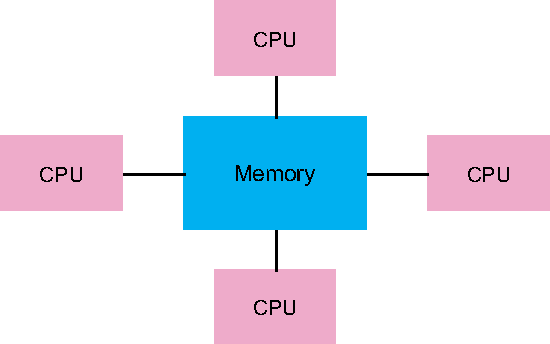
\includegraphics[width=0.42\linewidth]{fig/uma.pdf}%
		\label{uma}}
	\hspace{34.5pt}
	\subfloat[Shared Memory Architecture (NUMA)]{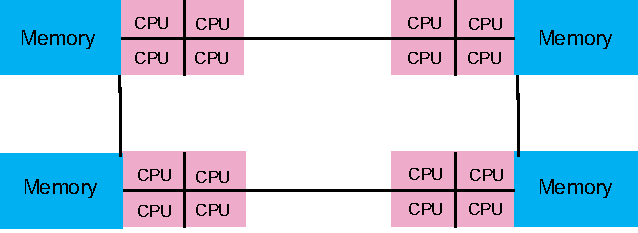
\includegraphics[width=0.42\linewidth]{fig/numa.pdf}%
		\label{numa}}
		\hspace{11.5pt}
		\subfloat[Distributed Memory Architectures.]{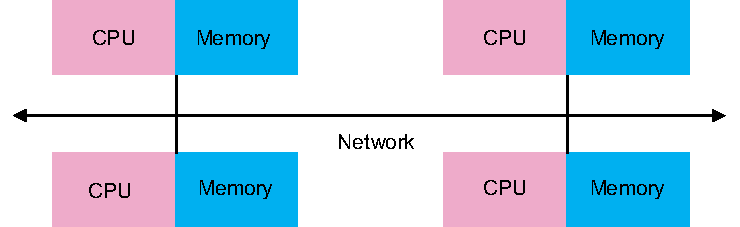
\includegraphics[width=0.464\linewidth]{fig/distributed.pdf}%
		\label{distributed}}
	\hspace{1.5pt}
	\subfloat[Distributed Shared Memory Architectures.]{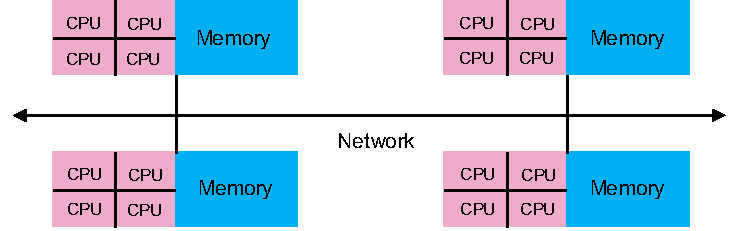
\includegraphics[width=0.464\linewidth]{fig/hybrid.pdf}%
		\label{hybrid}}
	\caption{Parallel Computer Memory Architectures.}
	\label{parallel-memory}
\end{figure}

Then the distributed-memory architecture is proposed, which takes many multicore computers and connects them using a network, much like workers in different offices communicating by telephone. With a sufficiently fast network, we can in principle extend this approach to millions of CPU-cores and beyond. As shown in Fig. \ref{distributed}, inside distributed memory system, processors have their local memory. Memory addresses in one processor do not map to another processor, so there is no concept of global address space across all processors. Because each processor has its local memory, it operates independently. Changes it makes to its local memory do not affect the memory of other processors. Hence, the concept of cache coherency does not apply. When a processor needs access to data in another processor, it is usually the task of the programmer to explicitly define how and when data is communicated. Synchronization between tasks is likewise the programmer's responsibility. The advantages of distributed memory architecture are: 
\begin{enumerate}
	\item Memory is scalable with the number of processors. Increase the number of processors and the size of memory increases proportionately; 
	\item Each processor can rapidly access its memory without interference and without the overhead incurred with trying to maintain global cache coherency;
	\item Cost effectiveness.
\end{enumerate}

The disadvantages are: 
\begin{enumerate}
	\item the programmer is responsible for many of the details associated with data communication between processors;
	\item it may be difficult to map existing data structures, based on global memory, to this memory organization;
	\item non-uniform memory access times - data residing on a remote node takes longer to access than local node.
\end{enumerate}

Nowadays, the largest and fastest computers in the world employ both shared and distributed memory architectures (shown as Fig. \ref{hybrid}). The shared memory component can be a shared memory machine and/or graphics processing units (GPU). The distributed memory component is the networking of multiple shared memory/GPU machines, which know only about their memory - not the memory on another computer. Therefore, network communications are required to move data from one machine to another. Current trends seem to indicate that this type of memory architecture will continue to prevail and increase at the high end of computing for the foreseeable future.

In a word, shared-memory systems are challenging to build but easy to use and are ideal for laptops and desktops. Distributed-shared memory systems are easier to build but harder to use, comprising many shared-memory nodes with their separate memory. Distributed-shared memory systems introduce much more hierarchical memory and computing with multi-level of parallelism. The critical advantage of distributed-shared memory architectures is increasing scalability, and the important disadvantage is increasing the complexity to the program.

\subsection{Nvidia GPGPU}

General-purpose computing on graphics processing units (GPGPU) is the use of a GPU, which typically handles computation only for computer graphics, to perform computation in applications traditionally handled by the CPU. Modern GPUs are very efficient at manipulating computer graphics and image processing. Due to its special functionality, GPGPU serves as an accelerator of CPU to improve the overall performance of computers. Nowadays, it is becoming increasingly common to use GPGPU to build the supercomputers. According to the newest top500 list of the November 2018, 5 of top 10 supercomputers in the world use GPGPU.

\begin{figure}[htbp]
	\centering
	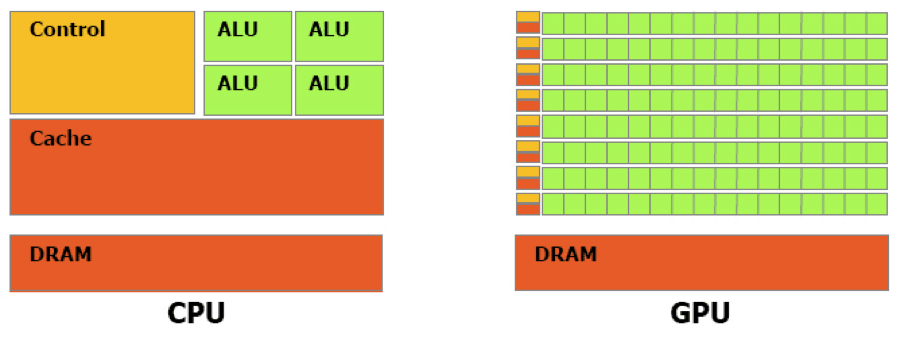
\includegraphics[width=0.99\linewidth]{fig/cpu_vs_gpu.png}
	\caption{CPU vs GPU architectures.}
	\label{cpuvsgpu}
\end{figure}

As shown in Figure \ref{cpuvsgpu}, the architectures of CPU and GPU are different: the CPU has a small number of complex cores and massive caches while the GPU has thousands of simple cores and small caches. The massive Arithmetic Logic Units (ALUs) of GPU are simple, data-parallel, multi-threaded which offer high computing power and large memory bandwidth. In brief, graphics chips are designed for parallel computations with lots of arithmetic operations, and CPUs are for general complex applications. The host character of CPU requires complicated cores and deep pipelines to deal with all kinds of operations. It usually runs at a higher frequency and supports branch prediction. The GPU only focuses on simple data-parallel operations thus the pipeline is shallow. The same instructions are used on large datasets in parallel with thousands of hardware cores, so the branch prediction is not necessary, and important arithmetic operations instead of caching hide memory access latency. GPGPU is also regarded as a powerful backup to overcome the \textit{power wall}.

Introduced in mid-2017, the newest \textit{Tesla V100} card can deliver $7.8$ TFLOPS in double-precision floating point (DP) and $15.7$ TFLOPS for single-precision (SP).

\subsection{Intel Many Integrated Cores}

The performance improvement of processors comes from the increasing number of computing units within the small chip area. Thanks to advanced semiconductor processes, more transistors can be built in one shared-memory system to do multiple things at once: from the view of programmers, this can be realized in two ways: different data or tasks execute in multiple individual computing units (multi-thread) or long uniform instruction decoders (vectorization).

\begin{figure}[htbp]
	\centering
	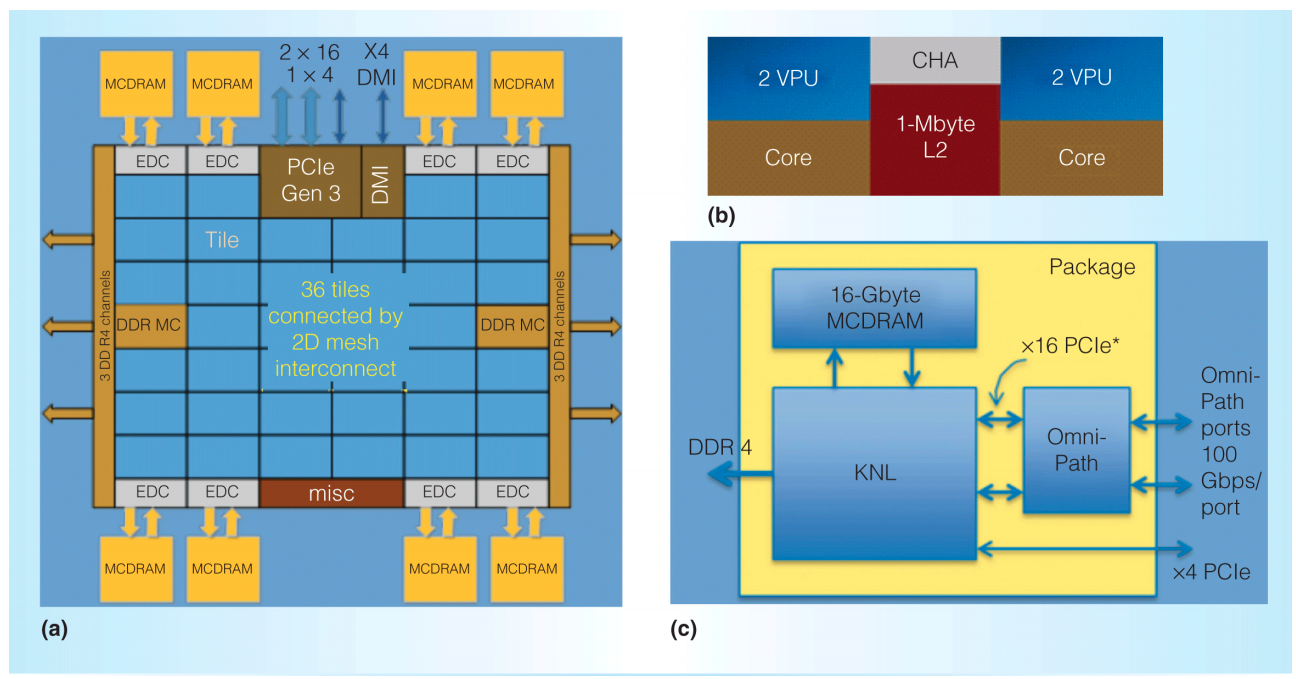
\includegraphics[width=0.99\linewidth]{fig/KNL1.png}
	\caption{The organization of a Intel Knights Landing processor.}
	\label{knl1}
\end{figure}

Intel officially first revealed the latest MIC codenamed \textit{Knights Landing (KNL)} in 2013. Being available as a coprocessor like previous boards, KNL can also serve as a self-boot MIC processor that is binary compatible with standard CPUs and boot standard OS. These second generation chips could be used as a standalone CPU, rather than just as an add-in card. Another key feature is the on-card high-bandwidth memory (HBM) which provides high bandwidth and large capacity to run large HPC workloads. Memory bandwidth is one of the common performance bottlenecks for computational applications due to the memory wall. KNL implements a two-level memory system to address this issue. The main difference between Xeon Phi and a GPGPU like Nvidia Tesla is that Xeon Phi, with an x86-compatible core, can, with less modification, run software that was originally targeted at a standard x86 CPU.

\subsection{RISC-based (Co)processors}

A reduced instruction set computer (RISC)  is such a machine has a small set of simple and general instructions, rather than a large set of complex and specialized instructions. A type of well-known RISC-based computing units are the ARM architecture processors. In the 21st century, the use of in smartphones and tablet computers provided a wide user base for RISC-based systems. Since the introduction of Sunway TaihuLight\footnote{http://www.nsccwx.cn/}, RISC processors are also used in supercomputers. RISC based supercomputers enable low energy consumption per core and cheaper chips since they do not contain complex instruction sets. In this section, we list two types of RISC based (co)processors for the supercomputers.

The first type of processor is sw26010, which is a 260-core manycore processor \cite{fu2016sunway} designed by the National High-Performance Integrated Circuit Design Center in Shanghai. It implements the Sunway architecture, a 64-bit RISC architecture designed by China. As shown in Fig. \ref{fig:sw26010}, the sw26010 has four clusters of 64 Compute-Processing Elements (CPEs) which are arranged in an eight-by-eight array. The CPEs support SIMD instructions and are capable of performing eight double-precision floating-point operations per cycle. Each cluster is accompanied by a more conventional general-purpose core called the Management Processing Element (MPE) that provides supervisory functions. Each cluster has its own dedicated DDR3 SDRAM controller and a memory bank with its own address space. The processor runs at a clock speed of 1.45.

\begin{figure}[t]
	\centering
	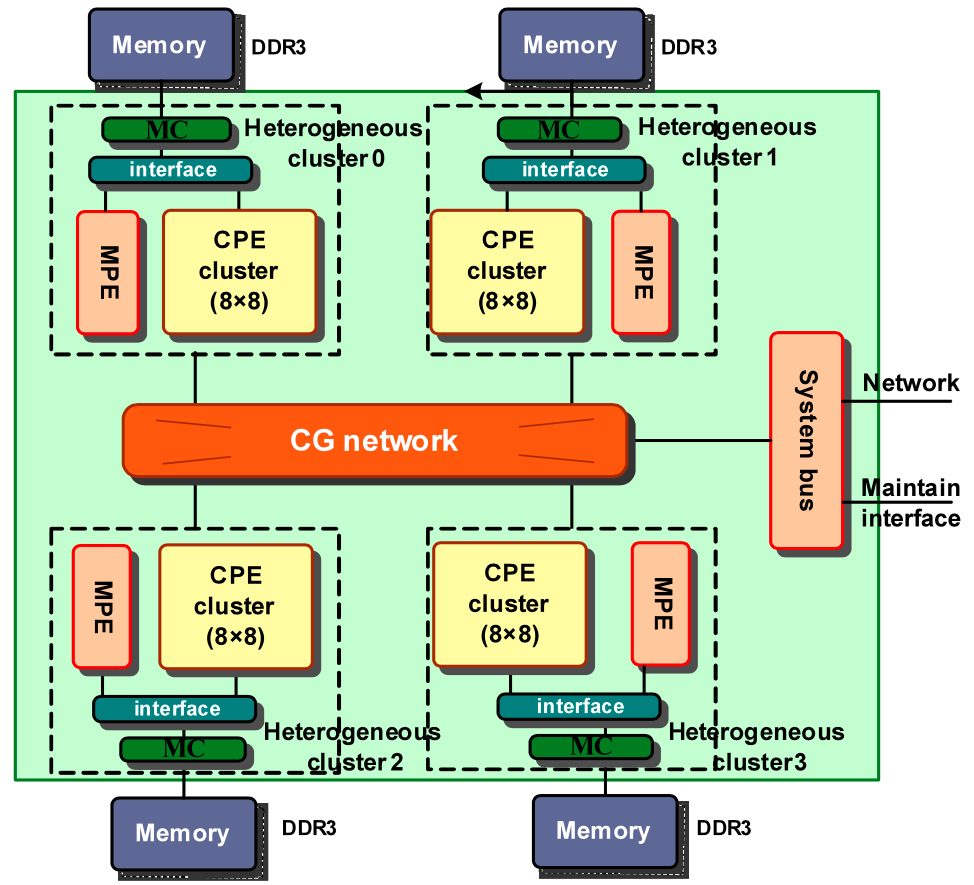
\includegraphics[width=0.81\linewidth]{fig/sw26010.png}
	\caption{The organization of a sw26010 manycore processor.}
	\label{fig:sw26010}
\end{figure}

Matrix-2000 \cite{matrix-2000} is a 64-bit 128-core many-core processor designed by NUDT and introduced in 2017. This chip was designed exclusively as an accelerator for China's Tianhe-2A supercomputer installed in the National Supercomputing Center in Guangzhou\footnote{http://www.nscc-gz.cn} in order to upgrade and replace the aging Intel's Knights Corner accelerators. The Matrix-2000 features 128 RISC cores operating at 1.2 GHz achieving 2.46/4.92 TFLOPS (DP/SP) with a peak power dissipation of 240W. The Matrix-2000 consists of 128 cores, eight DDR4 memory channels, and x16 PCIe lanes. The chip consists of four supernodes (SN) consisting of 32 cores each operating at 1.2 GHz with a peak power dissipation of 240 Watts.

\subsection{FPGA}

Field-programmable gate array (FPGA) is an integrated circuit designed to be configured: an array of programmable logic blocks and reconfigurable interconnects. The FPGA architecture provides the flexibility to create a massive array of application-specified ALUs that enable both instruction and data-level parallelism. FPGA has very high energy efficiency because it requires the low frequency and unused computing blocs do not consume energy. FPGAs can serve as accelerators on the supercomputers, e.g., Paderborn Center for Parallel Computing\footnote{https://pc2.uni-paderborn.de} installed several prototype hybrid machines by combining FPGAs with Intel Xeon CPUs. FPGAs are by no means anything new in the HPC sector – ten years ago they were all the rage but proved very difficult to program, and now they are coming back in vogue as it gets easier to C, C++, and Fortran applications to these devices.


\section{Parallel Programming Model}\label{Parallel Programming Model}

After the introduction of hardware architectures, this section presents the different levels of parallel programming models to develop applications on supercomputers. Most of the modern supercomputers are of distributed-shared memory architecture, which introduces multi-level parallel programming models, including the shared memory/thread level parallelism models, the distributed memory/process level parallelism models, the Partitioned Global Address Space (PGAS) models and the task/workflow based parallel models.

\subsection{Shared Memory Level Parallelism}

In this section, we introduce various runtimes developed to support the shared memory level parallelism of different computing architectures. 

\subsubsection{OpenMP}

OpenMP (Open Multi-Processing) \cite{dagum1998openmp} is an application programming interface (API) that supports multi-platform shared memory parallel programming in C, C++, and Fortran. OpenMP supports most platforms, instruction set architectures, and operating systems. It consists of a set of compiler directives, library routines, and environment variables. OpenMP provides the capability to incrementally parallelize a serial program with by inserting the specific directives. The compiler can ignore these directives, and the application can be executed in a sequential way when target machines do not support OpenMP. OpenMP is designed for multi-processor/core, shared memory machines. The underlying architecture can be shared memory UMA or NUMA. OpenMP programs accomplish parallelism exclusively through the use of threads.

\begin{figure}[htbp]
	\centering
	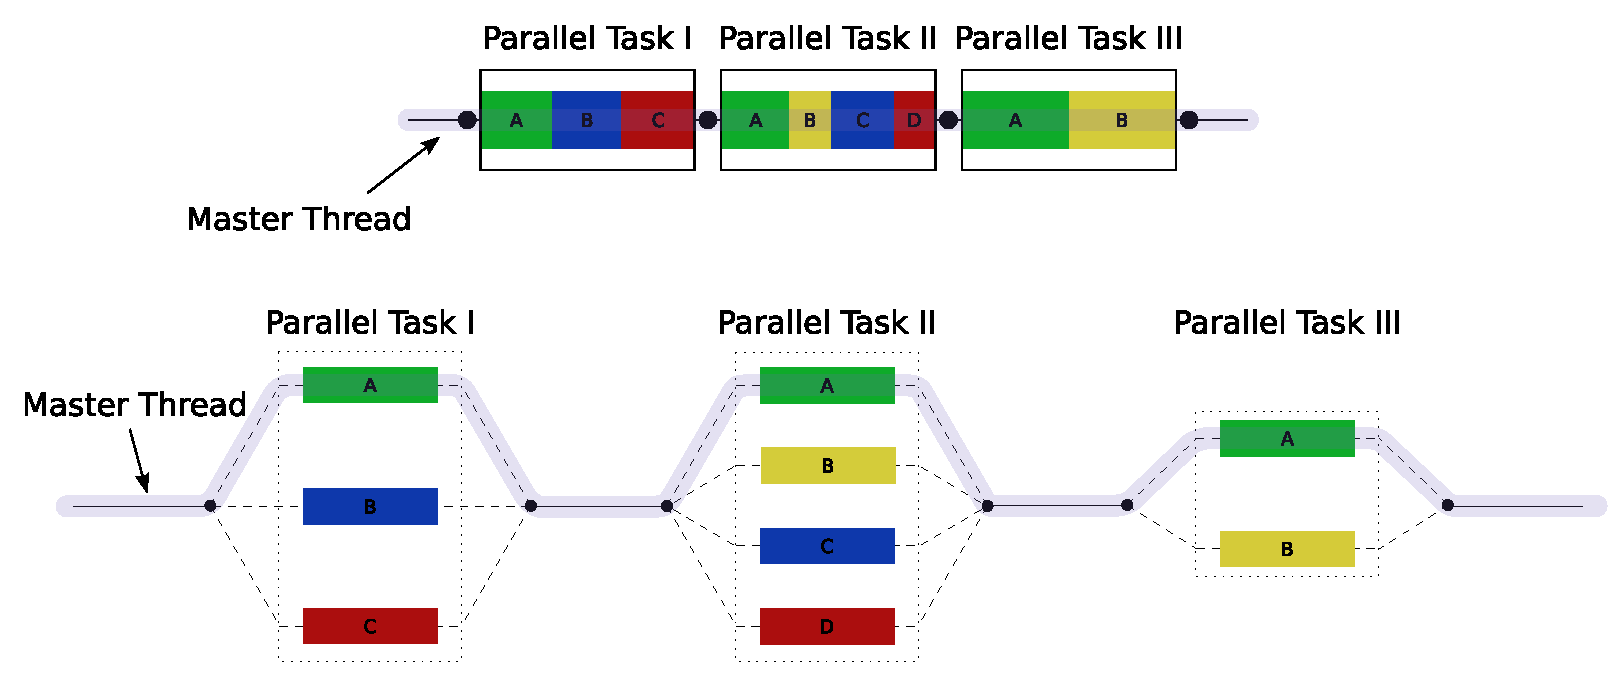
\includegraphics[width=6.4in]{fig/Fork_join.pdf}
	\caption{OpenMP \textit{fork-join} Model.}
	\label{openmp_fork_join}
\end{figure}

As shown in Fig. \ref{openmp_fork_join}, OpenMP uses the \textit{fork-join} model to support parallel execution. All OpenMP programs begin with a single process which executes until sequentially the first parallel region construct is encountered.  Then this thread creates a team of parallel threads and distributes the workload to them in order to have them work simultaneously. When the team threads complete the statements in the parallel region construct, they synchronize and terminate, leaving only the master thread. The new released OpenMP begins to support task scheduling strategies, the SIMD directives for high-level vectorization and the \textit{offload} directives for heterogeneous systems.

\subsubsection{CUDA}

CUDA (Compute Unified Device Architecture) \cite{nvidia2011nvidia} is a parallel programming platform and application programming interface model created by Nvidia. It allows software developers and engineers to use a CUDA-enabled GPU for general purpose processing. The CUDA software layer gives direct access to GPU's virtual instruction set and parallel computational elements, for the execution of compute kernels. The CUDA platform is designed to work with programming languages such as C, C++, and Fortran. This accessibility makes it easier for specialists in parallel programming to use GPU resources. Fig. \ref{cuda_flow} gives the four steps of processing flow on CUDA:

\begin{enumerate}
	\item Copy the processing data from main memory to memory for GPU;
	\item Load the executable from CPU to GPUs;
	\item Execute parallel the operations in each core;
	\item Copy back the results from memory for GPU to the main memory.
\end{enumerate}

\begin{figure}[htbp]
	\centering
	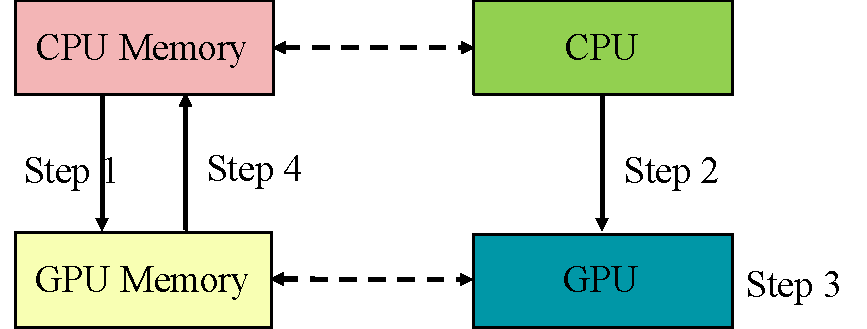
\includegraphics[width=0.72\linewidth]{fig/CUDA.pdf}
	\caption{Processing flow on CUDA.}
	\label{cuda_flow}
\end{figure}

\subsubsection{OpenCL}

OpenCL (Open Computing Language) \cite{munshi2009opencl} is a framework for writing programs that execute across heterogeneous platforms consisting of CPUs, GPUs, DSPs, FPGAs, and other processors or hardware accelerators. OpenCL specifies programming languages (based on C99 and C++11) for programming these devices and application programming interfaces (APIs) to control the platform and execute programs on the compute devices. OpenCL provides a standard interface for parallel computing using task- and data-based parallelism.

\subsubsection{OpenACC}

OpenACC (for open accelerators) \cite{wienke2012openacc} is a programming standard for parallel computing developed by Cray, CAPS, Nvidia and PGI. The standard is designed to simplify parallel programming of heterogeneous CPU/GPU systems. As in OpenMP, the programmer can annotate C, C++ and Fortran source code to identify the areas that should be accelerated using compiler directives and additional functions. Like OpenMP 4.0 and newer, OpenACC can target both the CPU and GPU architectures and launch computational code on them.

\subsubsection{Kokkos}

Kokkos \cite{edwards2014kokkos} core implements a programming model in C++ for writing performance portable applications targeting all major HPC platforms. For that purpose, it provides abstractions for both parallel executions of code and data management. Kokkos is designed to target complex node architectures with N-level memory hierarchies and multiple types of execution resources. It currently can use OpenMP, Pthreads, and CUDA as backend programming models.


\subsection{Distributed Memory Level Parallelism}

In the distributed memory platforms, each processor owns a private memory which is not reachable from other processors. The only way for processors to exchange data is to use explicit communication by sending and receiving messages. 

\subsubsection{Message Passing Interface}

MPI (Message Passing Interface) \cite{gropp1999using} is a standardized and portable message-passing standard designed by a group of researchers from academia and industry to support a wide variety of parallel computing architectures. MPI provides a simple-to-use portable interface for the basic user, yet one powerful enough to allow programmers to use the high-performance message passing operations available on advanced machines. Most MPI implementations consist of a specific set of routines directly callable from C, C++, Fortran and any language able to interface with such libraries.  MPI library functions include, but are not limited to, basic point-to-point send/receive operations, collective functions involving communication among all processes, synchronizing nodes (barrier operation), the one-sided communication, dynamic process management, I/O and so on. 

\begin{figure}[htbp]
	\centering
	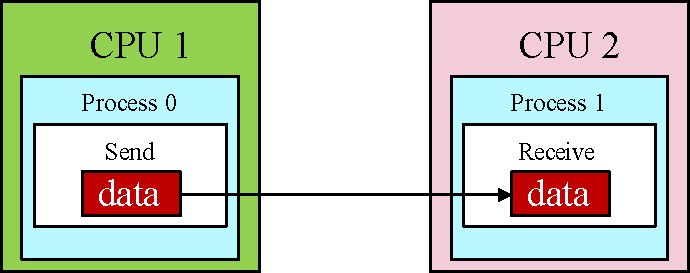
\includegraphics[width=0.72\linewidth]{fig/point-point.pdf}
	\caption{MPI point to point send and receive Model.}
	\label{mpi_model}
\end{figure}

As shown in Fig. \ref{mpi_model}, \textit{point-to-point operations} support the communication in both synchronous and asynchronous ways. Point-to-point operations, as these are called, are particularly useful in patterned or irregular communication, for example, a data-parallel architecture in which each processor routinely swaps regions of data with specific other processors between calculation steps, or a master-slave architecture in which the master sends new task data to a slave whenever the prior task is completed. MPI supports mechanisms for both blocking and non-blocking point-to-point communication mechanisms, as well as the so-called 'ready-send' mechanism whereby a send request can be made only when the matching receive request has already been made.

Collective functions (shown as Fig. \ref{mpi_collective}) involve communication among all processes in a process group (which can mean the entire process pool or a program-defined subset). A typical function is the MPI\_Bcast call (short for "broadcast"). This function takes data from one node and sends it to all processes in the process group. A reverse operation is the MPI\_Reduce call, which takes data from all processes in a group, operates (such as summing), and stores the results on one node. MPI\_Reduce is often useful at the start or end of a largely distributed calculation, where each processor operates on the part of the data and then combines it into a result. Fig. \ref{mpi_collective} gives six modes of collective communications, including broadcast, scatter, gather, reduction, all gather and all reduction.

\begin{figure}[t]
	\centering
	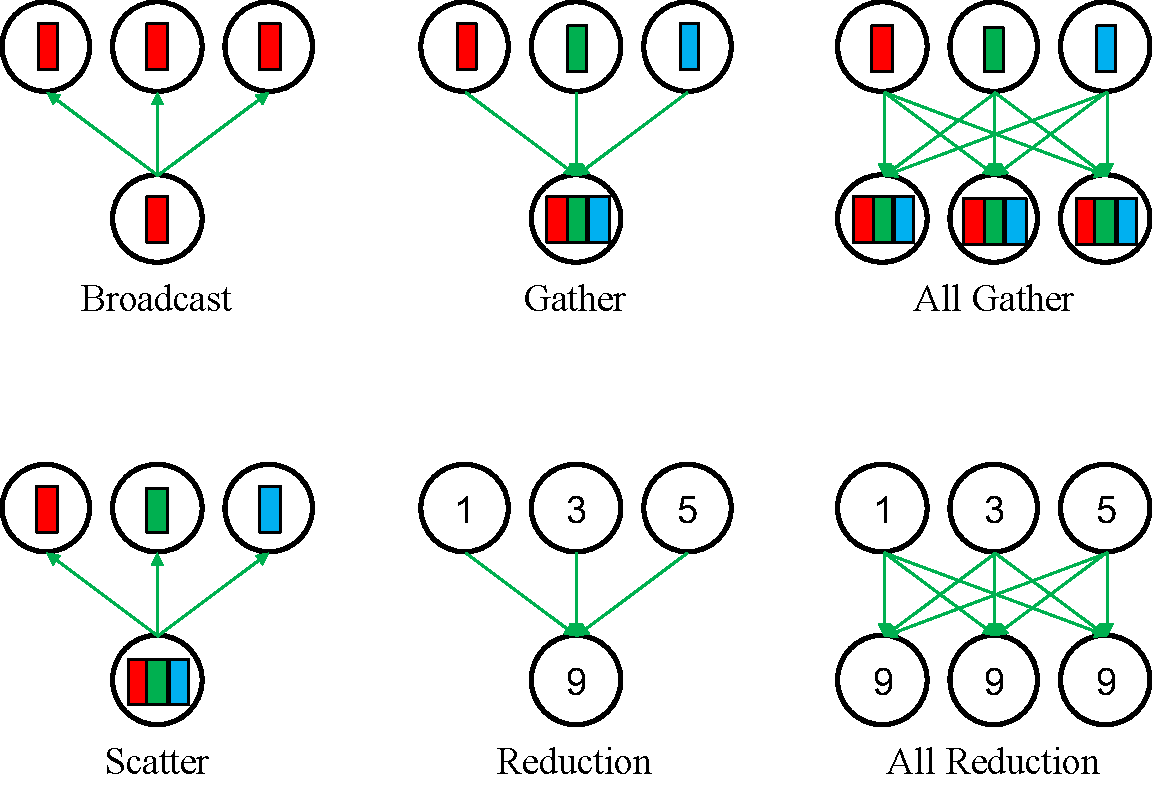
\includegraphics[width=0.99\linewidth]{fig/collective.pdf}
	\caption{Different modes of collective operations.}
	\label{mpi_collective}
\end{figure}

In modern computing platform with multiple shared-memory nodes, the shared memory programming models such as OpenMP and message passing programming such as MPI can be considered as complementary programming approaches, and can occasionally be used together in a hybrid way. This hybrid model is called \textit{MPI+X}.

\subsection{Partitioned Global Address Space}

In computer science, a partitioned global address space (PGAS) is a parallel programming model. Shown as Fig. \ref{fig:pgas}, it assumes a global memory address space that is logically partitioned and a portion of it is local to each process, thread, or processing element. The novelty of PGAS is that the portions of shared memory space may have an affinity for a particular process, thereby exploiting locality of reference. There are different implementation based on PGAS model, such as Unified Parallel C, Coarray Fortran, Chapel, X10, UPC++, DASH, XcalableMP, etc. PGAS attempts to combine the advantages of an SPMD programming style for distributed memory systems (as employed by MPI) with the data referencing semantics of shared memory systems. This is more realistic than the traditional shared memory approach of one flat address space because hardware-specific data locality can be modeled in the partitioning of the address space.

\begin{figure}[htbp]
	\centering
	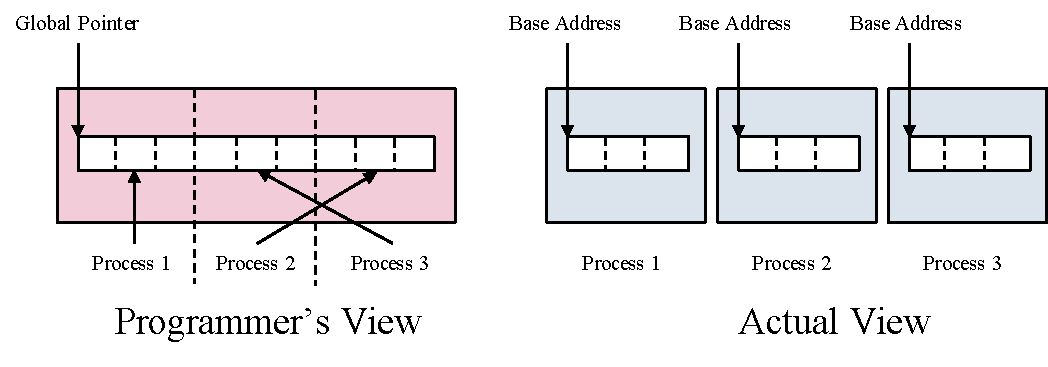
\includegraphics[width=6.3in]{fig/pgas.pdf}
	\caption{Programmer's and actual views of memory address in the PGAS languages.}
	\label{fig:pgas}
\end{figure}

\subsubsection{XcalableMP}

XcalableMP \cite{lee2010implementation} is a PGAS language extension of C and Fortran for parallel programming on distributed memory systems that help users to reduce those programming efforts. XcalableMP provides two programming models. 

\begin{itemize}
	\item \textit{Global view model}, which supports typical parallelization based on the data and task parallel paradigm, and enables parallelizing the original sequential code using minimal modification with simple, OpenMP-like directives. In the global view model, users specify the collective behavior of nodes in the target program to parallelize it. As users specify with the directives how data and computation are distributed on nodes, compilers are responsible for doing it. This model is suitable for regular applications, such as domain-decomposition problems, where every node works in a similar way.
	
	\item \textit{Local view model}, which allows using CAF-like expressions to describe inter-node communication. In the local-view mode, users specify the behavior of each node, just like MPI. Communications in this model can be specified in a one-sided manner based on coarrays. This model is suitable for applications where each node performs a different task.
\end{itemize}

XcabableMP supports both two-sided (MPI like) and one-sided (remote memory access) communications. Users can even use MPI and OpenMP explicitly in the XMP language to optimize performance explicitly.

\subsection{Task/Graph Based Parallel Programming}

With the increase of the complexity of applications on the supercomputers, it is more and more difficult for the developers to maintain the parallel codes on the modern computing architectures. The task/graph based parallel programming models are proposed to express the task parallelism and data dependencies of complex codes. An application can be divided temporally and spatially into inter-dependent tasks of different natures. A good scheduler can manage the complex tasks efficiently across a large number of cores on the supercomputing systems.  Fig. \ref{fig:workflow_cholesky} \cite{bosilca2012dague} gives the workflow of Cholesky factorization for a 4$\times$4 tile matrix on a 2$\times$2 grid of processors.

\begin{figure}[t]
	\centering
	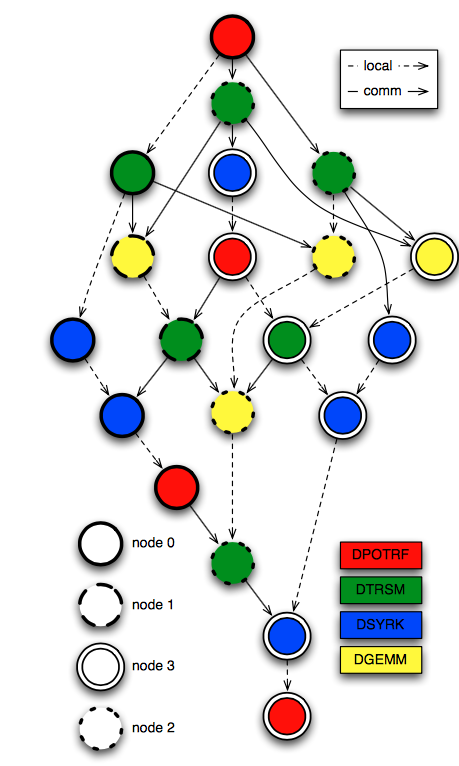
\includegraphics[width=0.5\linewidth]{fig/workflow_cholesky.png}
	\caption{Workflow of Cholesky for a 4$\times$4 tile matrix on a 2$\times$2 grid of processors. Figure by Bosilca et al. \cite{bosilca2012dague}}
	\label{fig:workflow_cholesky}
\end{figure}

The notion of granularity is introduced to describe the amount of work or task size that can be executed before communicating or synchronizing with others. The choice of grain size is important to the parallel applications. In fact, with coarse-grained tasks, there may not be enough of them to be executed in parallel.  In contrast,  a large number of fine-grained tasks will cause unnecessary parallel overhead.  Modern applications on supercomputers should consider multi-level granularities to fit in the hierarchical systems. In this section, we list several well-known task/graph based parallel programming runtime environments developed to support either coarse-grained or fine-grained tasks.

\subsubsection{StarPU}

StarPU\footnote{http://starpu.gforge.inria.fr} \cite{augonnet2011starpu} is a task programming library for hybrid architectures with shared memory. The application provides algorithms and constraints both the CPU/GPU implementations of tasks and the graphs of tasks, using either the StarPU's high-level GCC plugin pragmas, StarPU's rich C/C++ API, or OpenMP pragmas. StarPU handles runtime concerns: the task dependencies, the optimized heterogeneous scheduling, the optimized data transfers/replication between main memory and discrete memories and optimized cluster communications.

\subsubsection{OmpSs}

OmpSs\footnote{https://pm.bsc.es/ompss} is a task-based programming environment which covers both heterogeneous and homogeneous architectures. Its target is the programming of multi-GPU or many-core architectures and offers asynchronous parallelism in the execution of the tasks \cite{duran2011ompss}. OmpSs is build on top of Mercurium compiler\cite{balart2004nanos} and Nanos++ runtime system \cite{planas2013selection}. Nanos++ is able to schedule and run these tasks, taking care of the required data transfers and synchronizations on the accurate resources. Tasks in OmpSs are annotated with data directionality clauses that specify the use of data, and how it will be used (read, write or read \& write). Dependencies are then deduced at runtime from user-supplied annotations of data accesses which are translated into a format that can be exploited by Nanos++. Nanos++ proposes several scheduling policies which define how ready tasks are executed. 

%The most suitable scheduling policy can depend on the application and architecture used.

\subsubsection{YML}

YML\footnote{http://yml.prism.uvsq.fr} \cite{delannoyyml} allows users to transparently use one or more grid and supercomputer middlewares to run an application. YML can describe a complex parallel application regardless of the execution platform. The YvetteML language is used to express the task graph of the application. The nodes of the graph are the tasks described by components, and the edges correspond to dependencies or communications. The components are written in XML. Each component implementation can contain C++, XMP-C, XMP-FORTRAN or other code. Each component implementation can be expressed with finer grain parallelism. YML will be discussed in details in Chapter \ref{YML and XMP Multi-level Parallelism Programming Paradigm}.

\subsubsection{Swift}

Swift\footnote{http://swift-lang.org/main/index.php} \cite{wilde2011swift} is a data-flow oriented coarse-grained scripting language that supports dataset typing and mapping, dataset iteration, conditional branching, and procedural composition. Swift scripts are primarily concerned with processing (possibly large) collections of data files, by invoking programs to do that processing. Swift handles execution of such programs on remote sites by choosing sites, handling the staging of input and output files to and from the chosen sites and remote execution of programs.

\subsubsection{Legion}

Legion\footnote{http://legion.stanford.edu} \cite{grimshaw1994synopsis} is a data-centric parallel programming system for writing portable high performance programs targeted at distributed heterogeneous architectures. Legion presents abstractions which allow programmers to describe properties of program data (e.g., independence, locality). By making the Legion programming system aware of the structure of program data, it can automate many of the tedious tasks programmers currently face, including correctly extracting task- and data-level parallelism and moving data around complex memory hierarchies. A novel mapping interface provides explicit programmer controlled placement of data in the memory hierarchy and assignment of tasks to processors in a way that is orthogonal to correctness, thereby enabling easy porting and tuning of Legion applications to new architectures.

\section{Exascale Challenges of Supercomputers}\label{Exascale Challenges of Supercomputers}

The exscale computing era is coming, in this section, we analyze the trends of the increase of heterogeneity for modern supercomputers, and then summarize the challenges of parallel programming for exascale systems.

\subsection{Increase of Heterogeneity for Supercomputers} \label{Trends of Heterogeneity}

\begin{figure}[t]
	\centering
	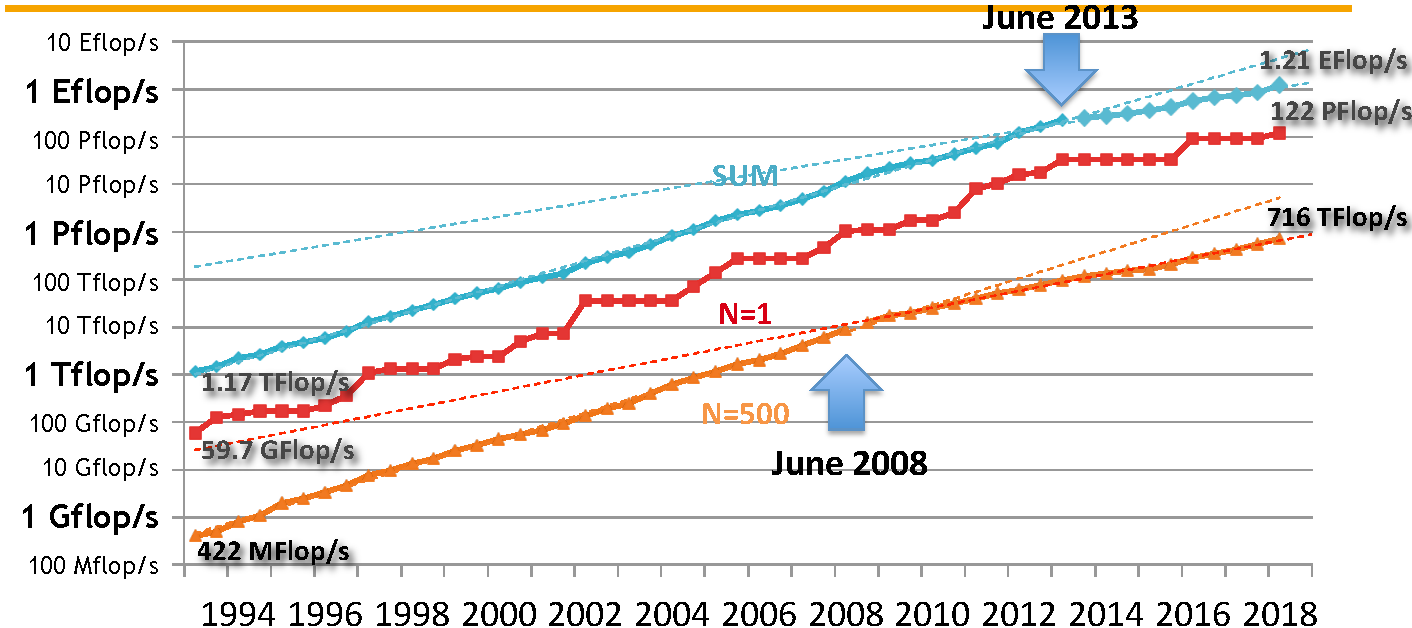
\includegraphics[width=0.99\linewidth]{fig/top500_2.pdf}
	\caption{HPL Performance in Top500 by year.}
	\label{hpc_evaluate}
\end{figure}

Hardware architectures have great impacts on the evolution of supercomputers. At the early age, the processor performance improves mainly by increasing the number of transistors per integrated circuit, According to \textit{Moore's law}, the number of transistors per integrated circuit doubles every $18$ months, which means that the size of the transistor is reduced to half, which allows achieving faster clock rate. Before 2002, \textit{Moore's law} was found to be totally acceptable. Since then, the overheating introduced by higher frequency reaches the limit of air cooling. This is the famous \textit{power wall}. Fig. \ref{hpc_evaluate} shows the HPL performance by year in Top500 List. \textit{Moore's law} is not totally acceptable in recent years, where the performance's evolution of supercomputer slows down. Since then, the modern computing architectures  trends to have multiple processors on-chip, lower operating frequency and hierarchical architectures come, including the GPGPU, Intel MIC, the many-core sw26010, and Matrix-2000 GPDSP, etc. Moreover, Europe (Mont-Blanc \cite{rajovic2016mont}, CEA and Atos \cite{ceaarm}) and Japan (RIKEN and Fujitsu) \cite{japanarm} are now pushing the development of ARM supercomputers. Fig. \ref{top500-acc} shows the trends of supercomputers equipped with accelerators by year. According to the Top 500 list of November 2018, 137 systems out of 500 use accelerator or co-processor technology. The introduction of accelerators on the supercomputers with a large number of cores increase their heterogeneity of communications, memory and computing units extremely.


\begin{figure}[t]
	\centering
	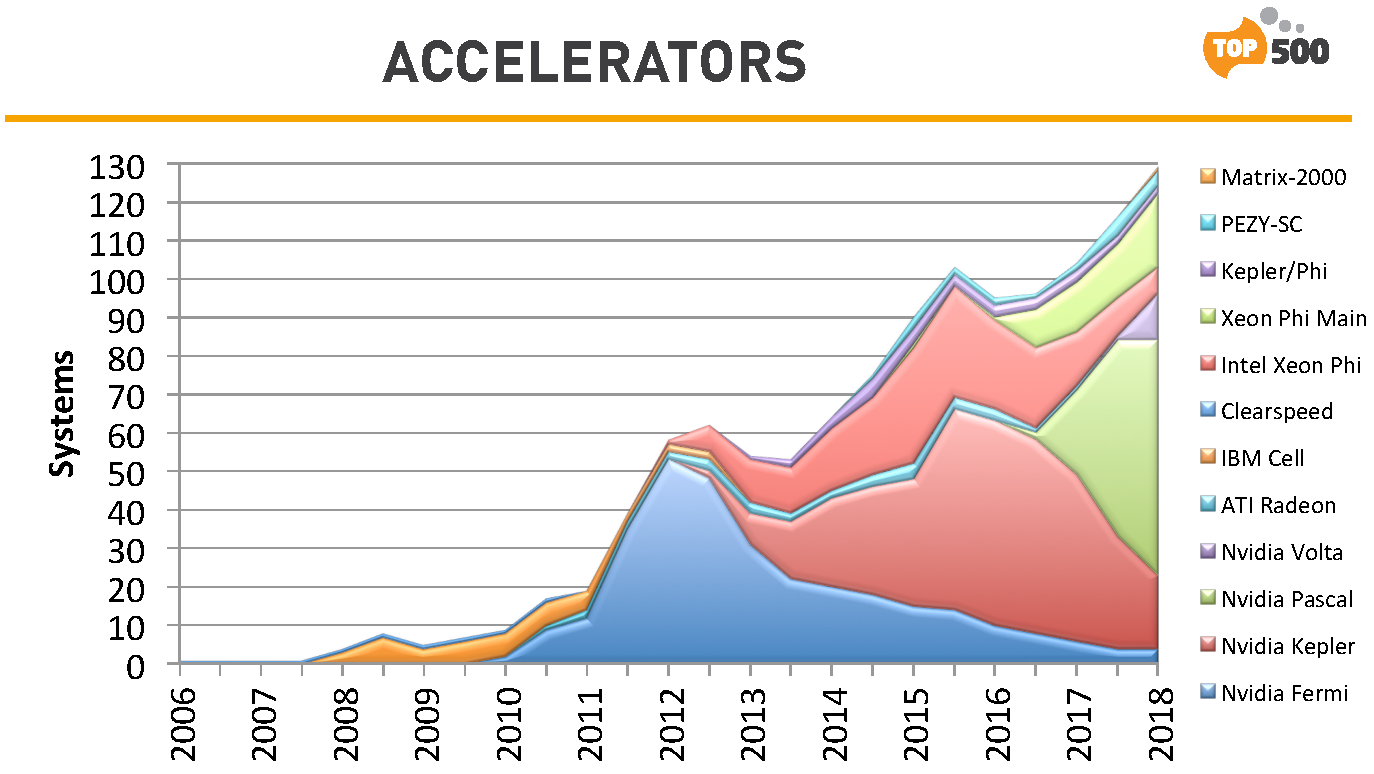
\includegraphics[width=0.99\linewidth]{fig/top500.pdf}
	\caption{Number of systems each year boosted by accelerators.}
	\label{top500-acc}
\end{figure}


Compared with the traditional computing architectures such as Intel, AMD CPUs which dedicate to multiple different purposes that result in lousy energy efficiency in HPC, the introduction of low frequency and/or less complex architecture improve the energy efficiency. In the Green500 list\footnote{https://www.top500.org/green500/} of November 2016, 8 out of 10 the most efficient supercomputers are equipped with the Nvidia GPGPU, and the No.1 machine of Green500 list \textit{ZettaScaler-2.2} installed by RIKEN is powered by the Intel low-frequency processor (\textit{Xeon D-1571 16C 1.3GHz}).

\subsection{Potential Architecture of Exascale Supercomputer} \label{Potential Architecture of Exascale Supercomputer}

This section tries to make a blueprint (shown as Fig. \ref{fig:supercomputer_arch}) for the upcoming exascale supercomputers based on the future architecture of Aurora Exascale system talked in \cite{TheNextPlatform}.

As shown in Fig. \ref{fig:supercomputer_arch}, the exascale supercomputers will be composed of more than 100,000 interconnected nodes (several million cores). Each compute node is packed with the thin cores and fat cores. The fat cores refer to the Intel, AMD X86 CPUs which dedicate to more complex operations. The thin cores can be the accelerators and co-processors (e.g., GPGPU, Matrix-2000, FPGA, etc.) with low frequency and/or less complex operations. A typical fat-thin mode is the Nvidia \textit{Host} and \textit{device} architecture. The fat cores are connected with RAM which has high capacity and low bandwidth, and the thin cores are connected with the memory which has low capacity and high bandwidth.

This fat core-thin core hybrid approach can also be found in the sw26010 processor deployed in the Sunway TaihuLight supercomputer. As shown in Fig. \ref{fig:sw26010}, this processor is designed with one fat core (MPE) which provides supervisory functions, and four auxiliary meshes of skinny cores  (CPEs) conducted to computing operations, each with 64 cores, for a total of 260 cores.

\begin{figure}[htbp]
	\centering
	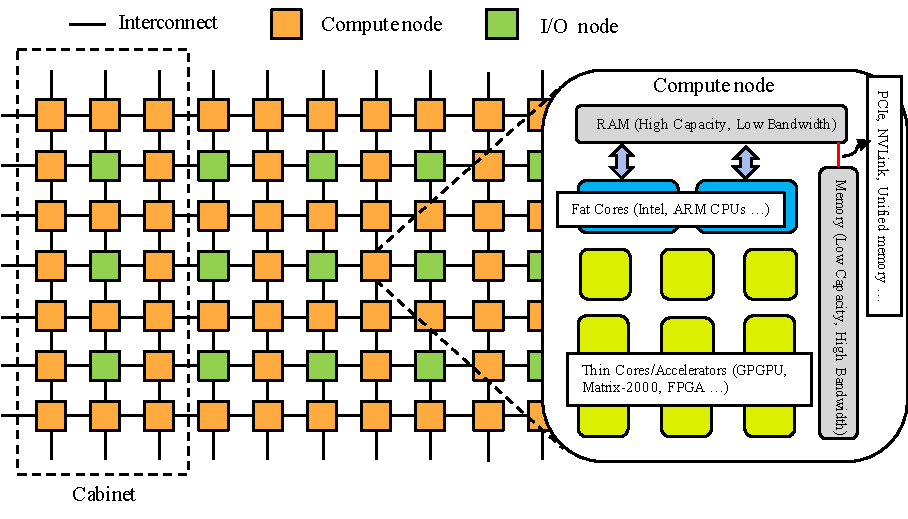
\includegraphics[width=0.99\linewidth]{fig/supercomputer_arch.pdf}
	\caption{Multi-level parallelism and hierarchical architectures in supercomputers.}
	\label{fig:supercomputer_arch}
\end{figure}

These hierarchical computing architectures introduces multiple level parallelism:

\begin{enumerate}
	\item $1^{st}$ level is the \textit{inter-node parallelism} between compute nodes: MPI is the considered model to manage the communication among the compute nodes, manager engine or other complex software stacks are required to handle huge traffic and failure of applications;
	\item $2^{nd}$ level is the \textit{intra-node parallelism}, including:
	\begin{itemize}
		\item shared memory parallelism with NUMA among cores and/or sockets in each compute node;
		\item heterogeneous computing with different accelerators, memory space, and bandwidth;
	\end{itemize}
	\item $3^{rd}$ level are the \textit{vectorization} techniques, which can compute a full vector of data with the same set of operations simultaneously. These techniques include the Single Instruction Multiple Data (SIMD) vectorization on CPUs, and the Single Instruction Multiple Thread (SIMT) vectorization, etc.
\end{enumerate}

\subsection{Parallel Programming Challenges} \label{Parallel Programming Challenges}

With the increase of the number of cores and compute nodes in the supercomputers, time spent in communication will overcome the computational time, and it becomes a great bottleneck for the modern applications to take advantages of supercomputers. Facing the challenges, the parallel programming should consider the highly hierarchical architectures of computation and memory, the increasing levels and degrees of parallelism, the heterogeneity of computing, memory, and scalability. HPL benchmark is a little out of date, which cannot represent the common operations on modern supercomputers.

\begin{figure}[htbp]
	\centering
	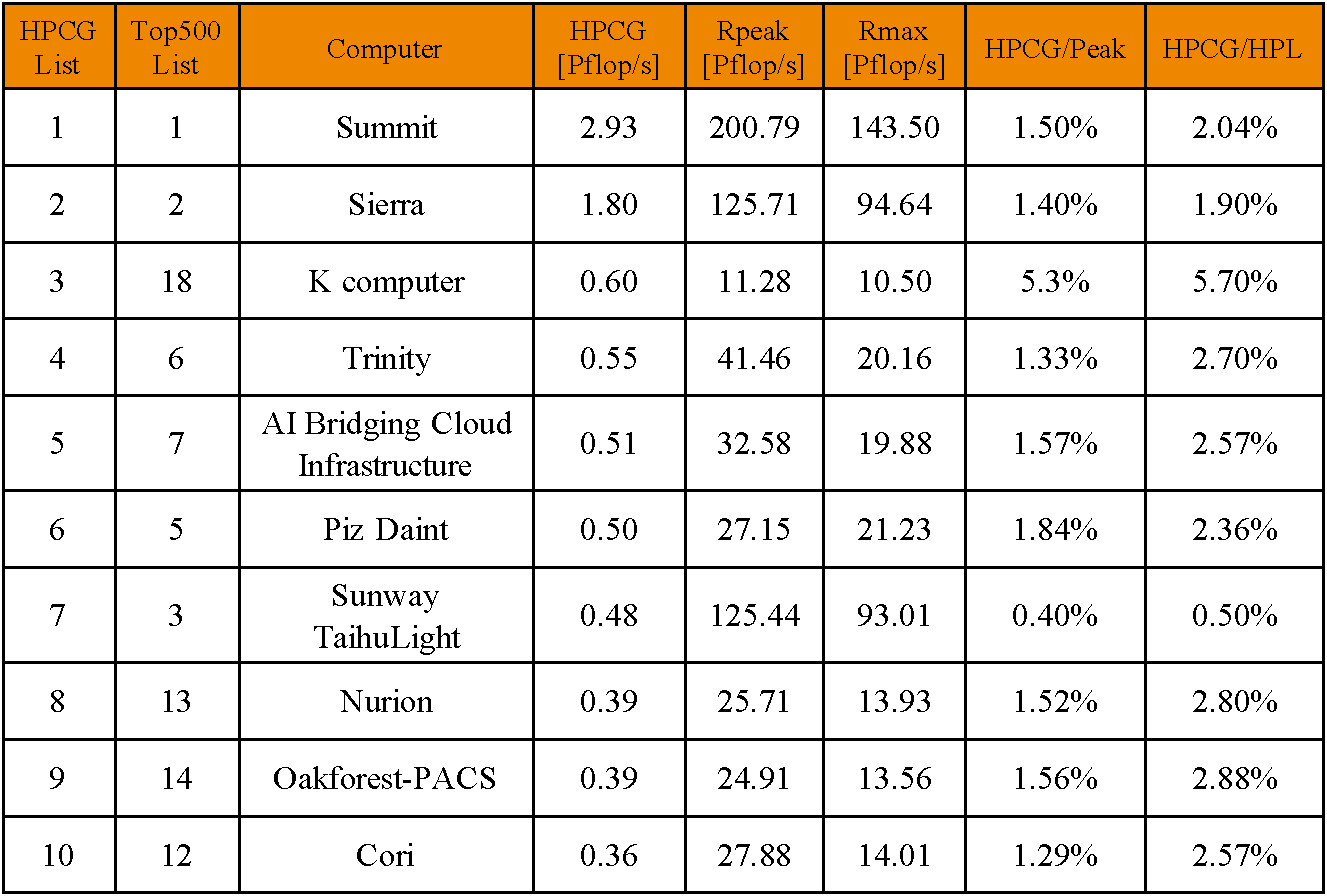
\includegraphics[width=0.99\linewidth]{fig/top500_hpcg.pdf}
	\caption{Top10 HPCG list of the November 2018.}
	\label{top500-hpxg}
\end{figure}

Thus, the High-Performance Conjugate Gradients (HPCG) Benchmark \cite{dongarra2015hpcg} was proposed by Dongarra et al. in 2015. In mathematics, the Conjugate Gradient (CG) method is an algorithm for the numerical solution of particular linear systems, namely those whose matrix is symmetric and positive-definite. These linear systems are general modeled  by Partial Differential Equations (PDE)  for the simulations of many aspects of the physical world, and CG can be seen as a good representive of modern applications on the supercomputers. HPCG project is an effort to create a new metric for ranking HPC systems, which is intended as a complement to HPL benchmark. The computational and data access patterns of HPL are still representative of some important scalable applications, but not all. HPCG is designed to exercise computational and data access patterns that more closely match a different and broad set of important applications, and to give incentive to computer system designers to invest in capabilities that will have the impact on the collective performance of these applications.

HPCG is a complete, stand-alone code that measures the performance of basic operations in a unified code:

\begin{itemize}
	\item Sparse matrix-vector multiplication.
	\item Vector updates.
	\item Global dot products.
	\item Local symmetric Gauss-Seidel smoother.
	\item Sparse triangular solve (as part of the Gauss-Seidel smoother).
	\item Driven by multigrid preconditioned conjugate gradient algorithm that exercises the key kernels on a nested set of coarse grids.
	\item Reference implementation is written in C++ with MPI and OpenMP support.
\end{itemize}

Fig. \ref{top500-hpxg} lists the Top10 computers in the HPCG List of November 2018.  We could conclude that the HPCG test generally achieves only an extremely tiny fraction of the peak FLOPS of the computers. Lots of modern algorithms are much more complex than the HPCG, and their parallel performance tends to be even worse. Thus,  the programming paradigm for parallel applications should be re-considered and re-designed.

In fact, with the increase of heterogeneity of supercomputers, HPC tends to be a little similar with the Grid computing, which is the use of widely distributed computer resources connected to a network (private, public or the Internet) to reach a common goal. Grid computing is distinguished from HPC systems in that grid computers have each node set to perform a different task/application. The geographically dispersed of Grid computers leads in many heterogeneous properties comparing with HPC systems. Since its heterogeneity, coordinating applications of Grid computing can be a complex task, especially when coordinating the flow of information across distributed computing resources. Hence workflow management systems have been developed specifically to compose and execute a series of computational or data manipulation steps, or a workflow. Current parallel applications can be seen as the intersection of distributed and parallel computing.

The parallel performance of a common application in HPC is measured by the scalability (also referred as the scaling efficiency). This measurement indicates how efficient an application is when using increasing numbers of parallel processing elements (CPUs/cores/processes/threads, etc.). There are two basic ways to measure the parallel performance of a given application, depending on whether or not one is CPU-bound or memory-bound. These are referred to as strong and weak scaling, respectively: 

\begin{itemize}
	\item  \textit{strong scaling} which is defined as how the solution time varies with the number of processors for a fixed total problem size;
	\item \textit{weak scaling} which is defined as how the solution time varies with the number of processors for a fixed problem size per processor.
\end{itemize}

In order to improve the parallel performance and get the best scaling efficiency on modern supercomputers, several principles should be considered for the development of applications:

\begin{enumerate}
	\item Algorithms should have multi-grains of parallelism to fit in the heterogeneity of computer architectures.
	\item Applications should be able to adapt to the hierarchical memory on supercomputers.
	\item The data movements should be limited, and the number of global communications should be minimized.
	\item The parallel programming should reduce synchronizations and promote the asynchronicity;
	\item Multi-level scheduling strategies should be proposed,  and the manager engine or other complex software stacks should be implemented to handle huge traffic and improve the fault tolerance and resilience, similarly as for Grid computing.
\end{enumerate}

In following chapters, we focus on the work of design and implementation of novel numerical methods for modern supercomputers based on these principles.

\clearemptydoublepage